\documentclass[11pt,letterpaper, leqno]{article}
\usepackage{latexsym}
\usepackage{amsmath}
\usepackage{amssymb}
\usepackage{amsthm}
\usepackage{enumerate}
\topmargin -0.25in
\textheight 8.5in
\oddsidemargin 0.0in
\textwidth 6.5in

\RequirePackage{amsthm,amsmath,amsfonts,amssymb}
%\RequirePackage[numbers]{natbib}
\RequirePackage[authoryear]{natbib}%% uncomment this for author-year citations
\RequirePackage[colorlinks,citecolor=blue,urlcolor=blue]{hyperref}%% uncomment this for coloring bibliography citations and linked URLs
\RequirePackage{graphicx}%% uncomment this for including figures

\usepackage{natbib}
\usepackage{authblk}
\usepackage[english]{babel}
\bibliographystyle{abbrvnat}
\setcitestyle{authoryear,open={(},close={)}}

% For the algorithm table
\usepackage{algorithm,algcompatible,amsmath}
\DeclareMathOperator*{\argmax}{\arg\!\max}
\DeclareMathOperator*{\argmin}{\arg\!\min}
% https://tex.stackexchange.com/q/83169/5764
\algnewcommand\INPUT{\item[\textbf{Input:}]}%
\algnewcommand\OUTPUT{\item[\textbf{Output:}]}%
%

\newtheorem{theorem}{Theorem}
\newtheorem{acknowledgement}[theorem]{Acknowledgement}
%\newtheorem{algorithm}[theorem]{Algorithm}
\newtheorem{axiom}[theorem]{Axiom}
\newtheorem{problem}[theorem]{Problem}
\newtheorem{remark}{Remark}
\newtheorem{claim}[theorem]{Claim}
\newtheorem{conclusion}[theorem]{Conclusion}
\newtheorem{condition}[theorem]{Condition}
\newtheorem{conjecture}[theorem]{Conjecture}
\newtheorem{corollary}{Corollary}
\newtheorem{criterion}[theorem]{Criterion}
\newtheorem{definition}{Definition}
\newtheorem{example}{Example}
\newtheorem{exercise}[theorem]{Exercise}
\newtheorem{lemma}{Lemma}
\newtheorem{proposition}{Proposition}
\newtheorem{thm}{Theorem}[section]
\newtheorem{lem}{Lemma}[section]
\newtheorem{prop}{Proposition}[section]
\newtheorem{defn}{Definition}[section]
\newtheorem{ex}{Example}[section]
\newtheorem{cor}{Corollary}[section]
\newtheorem{rem}{Remark}[section]
\newtheorem{rems}{Remarks}[section]
\numberwithin{equation}{section} 
\numberwithin{theorem}{section}
\numberwithin{lemma}{section} 
\numberwithin{corollary}{section}
\numberwithin{definition}{section}
\numberwithin{proposition}{section} 
\numberwithin{remark}{section}
\numberwithin{example}{section}
\newtheorem{assumption}{Assumption}
\DeclareMathOperator\supp{supp}

%\newcommand{\ex}{{\bf\sf E}}            %% expectation
\newcommand{\bfp}{{\bf P}}
\newcommand{\bfr}{{\bf R}}
\newcommand{\Var}{{\rm Var}}            %% 
\newcommand{\Cov}{{\rm Cov}}            %% 
\newcommand{\calc}{{\cal C}}            %%
\newcommand{\cald}{{\cal D}} 
\newcommand{\calf}{{\cal F}}            %%
\newcommand{\call}{{\cal L}}            
\newcommand{\al}{\alpha}                %%
\newcommand{\bt}{\beta}                %%
\newcommand{\ga}{\gamma}                %% abbreviated
\newcommand{\dt}{\delta}                %% greek letters
\newcommand{\la}{\lambda}               %%
\newcommand{\ep}{\epsilon}              %%
\newcommand{\sig}{\sigma}               %%
\newcommand{\tri}{\triangle}
\newcommand{\om}{\omega}                %%
\newcommand{\ra}{\rightarrow}           %%
\newcommand{\lra}{\longrightarrow}
\newcommand{\Ra}{\Rightarrow}           %% arrows
\newcommand{\subs}{\subseteq}           %% subset or equal to
\newcommand{\eqdef}{\stackrel{\triangle}{=}}
\newcommand{\hY}{\hat{Y}}
\newcommand{\hp}{\hat{p}}
\newcommand{\hX}{\hat{X}}
\newcommand{\hy}{\hat{y}}
\newcommand{\hQ}{\hat{Q}}
\newcommand{\Zh}{\hat{Z}}
\newcommand{\hla}{\hat{\lambda}}
\newcommand{\starti}{\parindent0pt\it}  %% start an italic line
\newcommand{\startb}{\parindent0pt\bf}  %% start a boldface line
\newcommand{\tril}{\triangle^-}
\newcommand{\trir}{\triangle^+}
\newcommand{\trilr}{\triangle^{\pm}}
\newcommand{\realR}{{{\rm I}\;\!\!\!{\rm R}}}
\newcommand{\probP}{{{\rm I}\;\!\!\!{\rm P}}}
\newcommand{\filtF}{{{\rm I}\;\!\!\!{\rm F}}}
\newcommand{\expeE}{{{\rm I}\;\!\!\!{\rm E}}}
\newcommand{\noin}{{\noindent}}
\newcommand{\doty}{{\dot{y}}}
\newcommand{\doth}{{\dot{h}}}
\newcommand{\dotx}{{\dot{x}}}
\newcommand{\dotu}{{\dot{u}}}
\newcommand{\dotf}{{\dot{f}}}
\newcommand{\dotg}{{\dot{g}}}
\newcommand{\ddoty}{{\ddot{y}}}
\newcommand{\ddoth}{{\ddot{h}}}
\newcommand{\ddotx}{{\ddot{x}}}
\newcommand{\ddotf}{{\ddot{f}}}
%\newcommand{\Var}{{\mbox{Var}}}
%\newcommand{\Cov}{{\mbox{Cov}}}

\renewcommand{\L}[1]{\mathcal{L}\{#1\}}
\newcommand{\ans}[1]{\boxed{\text{#1}}}
\newcommand{\vecs}[1]{\langle #1\rangle}
\renewcommand{\hat}[1]{\widehat{#1}}
\newcommand{\F}[1]{\mathcal{F}(#1)}
\renewcommand{\P}{\mathbb{P}}
\newcommand{\R}{\mathbb{R}}
\renewcommand{\qed}{\quad \blacksquare}
\newcommand{\brak}[1]{\langle #1 \rangle}
\newcommand{\E}{\mathbb{E}}
\newcommand{\bbm}[1]{\mathbbm{#1}}
\newcommand{\ind}{\mathbbm{1}}
\newcommand{\ellipsis}{\; \dots, \;}
\renewcommand{\Var}{\text{Var}\;}
\newcommand{\mfX}{\mathfrak{X}}
\newcommand{\Z}{\mathbb{Z}}

\newenvironment{solution}
  {\renewcommand\qedsymbol{$\blacksquare$}\begin{proof}[Solution]}
  {\end{proof}}

\usepackage{listings}
\usepackage{xcolor}
\usepackage{fancyhdr}
\usepackage{bbm}

\definecolor{codegreen}{rgb}{0,0.6,0}
\definecolor{codegray}{rgb}{0.5,0.5,0.5}
\definecolor{codepurple}{rgb}{0.58,0,0.82}
\definecolor{backcolour}{rgb}{0.95,0.95,0.92}

\lstdefinestyle{mystyle}{
    backgroundcolor=\color{backcolour},   
    commentstyle=\color{codegreen},
    keywordstyle=\color{magenta},
    numberstyle=\tiny\color{codegray},
    stringstyle=\color{codepurple},
    basicstyle=\ttfamily\footnotesize,
    breakatwhitespace=false,         
    breaklines=true,                 
    captionpos=b,                    
    keepspaces=true,                 
    numbers=left,                    
    numbersep=5pt,                  
    showspaces=false,                
    showstringspaces=false,
    showtabs=false,                  
    tabsize=2
}

\lstset{style=mystyle}

\begin{document}
\begin{center}
{\bf \Large APMA1690: ~~Homework \# 4 ~~~(Due by 11pm Oct 19)}
\end{center}
\[\]
\medskip

\section{Review}

Please read the review section before delving into the problem set.

\subsection{Random Variables}

Let $\boldsymbol{X}=(X^{(1)}, X^{(2)},\ldots,X^{(d)})$ be a $\mathbb{R}^d$-valued random variable defined on the probability space $(\Omega,\mathbb{P})$, i.e.,
\begin{align*}
    \boldsymbol{X}: \ \ & \Omega\rightarrow\mathbb{R}^d, \\
    & \omega \mapsto \boldsymbol{X}(\omega)=\Big(X^{(1)}(\omega), X^{(2)}(\omega), \ldots, X^{(d)}(\omega)\Big),
\end{align*}
where each $X^{(i)}$ is a $\mathbb{R}^1$-valued random variable. When $d>1$, $\boldsymbol{X}$ is also referred to as a ``random vector."

Suppose $H$ is a $d$-variable function which takes values in $\mathbb{R}$, i.e., 
\begin{align*}
    H:\ \ & \mathbb{R}^d \rightarrow \mathbb{R}, \\
    & \boldsymbol{x}=(x_1, x_2,\ldots,x_d) \mapsto H(\boldsymbol{x})=H(x_1, x_2,\ldots,x_d).
\end{align*}
Then, we have the $\mathbb{R}^1$-valued random variable $H(\boldsymbol{X})$ defined as follows
\begin{align*}
    H(\boldsymbol{X}): \ \ & \Omega\rightarrow\mathbb{R}^1, \\
    & \omega \mapsto H\left(\boldsymbol{X}(\omega)\right)=H\Big(X^{(1)}(\omega), X^{(2)}(\omega), \ldots, X^{(d)}(\omega)\Big).
\end{align*}

\subsection{Setup}

Suppose our goal is to compute the following multiple integral\footnote{We assume that all means and variances utilized herein do exist.}
\begin{align*}
    v=\int H(\boldsymbol{x}) \,d\boldsymbol{x} = \int_{-\infty}^\infty \cdots \int_{-\infty}^\infty H(x_1, x_2, \ldots, x_d) \,dx_1 dx_2\cdots dx_d,
\end{align*}
where $\boldsymbol{x}=(x_1, x_2, \ldots, x_d)$ and $d\boldsymbol{x}=dx_1 dx_2 \cdots dx_d$. This integral can be represented as follows
\begin{align*}
    \boxed{v=\int H(\boldsymbol{x}) \,d\boldsymbol{x}= \int \frac{H(\boldsymbol{x})}{f(\boldsymbol{x})}\cdot f(\boldsymbol{x}) \,d\boldsymbol{x}=\mathbb{E}\left[\frac{H(\boldsymbol{X})}{f(\boldsymbol{X})}\right],}
\end{align*}
where $f(\boldsymbol{x})$ is a $d$-dimensional PDF, and the random vector $\boldsymbol{X}=(X^{(1)}, X^{(2)}, \ldots, X^{(d)})\sim f(\boldsymbol{x})$. Additionally, the PDF $f(\boldsymbol{x})$ satisfies the following conditions
\begin{enumerate}
    \item $\{\boldsymbol{x}\in\mathbb{R}^d\,\vert\, H(\boldsymbol{x})\ne 0\} \subset \{\boldsymbol{x}\in\mathbb{R}^d\,\vert\, f(\boldsymbol{x})\ne 0\}$;
    
    \item We know how to generate random vectors $\boldsymbol{X}_1, \boldsymbol{X}_2,\ldots, \boldsymbol{X}_n \overset{iid}{\sim} f(\boldsymbol{x})$;
    
    \item $f(\boldsymbol{x})$ is similar to the ``optimal" PDF $\frac{1}{\int H(\boldsymbol{x}') d\boldsymbol{x}'} \cdot H(\boldsymbol{x})$. This similarity makes $\operatorname{Var}\left(\frac{H(\boldsymbol{X}_1)}{f(\boldsymbol{X}_1)}\right)$ small. (Since the integral $v=\int H(\boldsymbol{x}') d\boldsymbol{x}'$ is unavailable at this point, the optimal PDF is not achievable.)
\end{enumerate}

\subsection{Importance Sampling}

We generate random vectors $\boldsymbol{X}_1, \boldsymbol{X}_2,\ldots, \boldsymbol{X}_n \overset{iid}{\sim} f(\boldsymbol{x})$ and compute the following estimator of $v$
\begin{align}\label{eq: importance sampling estimator}
    \boxed{ \widehat{v}_n=\frac{1}{n}\sum_{i=1}^n \left[\frac{H(\boldsymbol{X}_i)}{f(\boldsymbol{X}_i)}\right]. }
\end{align}
Then, we have
\begin{enumerate}
    \item Law of large numbers $\implies$ $\widehat{v}_n\approx v$ when the sample size $n$ is sufficiently large;
    
    \item Law of the iterated logarithm $\implies$ $\vert \widehat{v}_n - v \vert \le \sqrt{\operatorname{Var}\left(\frac{H(\boldsymbol{X}_1)}{f(\boldsymbol{X}_1)}\right)} \cdot \sqrt{\frac{2\log(\log n)}{n}}$, where ``$\le$" holds in an approximate way. 
\end{enumerate}

A good reference for importance sampling is Chapter 7 of \cite{wang2012monte}.


\subsection{Markov Chains}

\textbf{Roughly speaking, a Markov chain is a sequence of random variables $\{X_n\}_{n=0}^\infty$ satisfying the Markov property.}\footnote{ For Markov chains in this course, we always let the index $n$ go from $0$ instead of $1$. It is just a convention.} In APMA 1690, we assume that all random variables take values in a generic \href{https://en.wikipedia.org/wiki/Countable_set}{countable set} $\mathcal{X}$, i.e., $\mathcal{X}$ can be expressed as $\mathcal{X}=\{\xi_0, \xi_1,\ldots, \xi_n,\ldots\}$. The countability assumption of $\mathcal{X}$ heavily simplifies the theory of Markov chains. The following is the definition\footnote{ The definition herein works only for the scenario where a Markov chain takes values in a countable space $\mathcal{X}=\{\xi_0, \xi_1,\ldots, \xi_n,\ldots\}$. It is one of the reasons that we assume $\mathcal{X}$ is countable. For the general definition of Markov chains and the relevant details, see Definition 17.1 and Remark 17.2 of \cite{klenke2013probability}. Since the materials of general Markov chains involve too much real analysis knowledge (see APMA 2110), we skip the general Markov chains in this course.} of Markov chains.
\begin{definition}
\begin{itemize}
    \item A sequence of random variables $\{X_n\}_{n=0}^\infty$ taking values in $\mathcal{X}$ is called a \textbf{Markov chain} if this sequence satisfies
\begin{align}\label{eq: Markov property for general MC}
    \boxed{ \mathbb{P}(X_{n+1}=y \,\vert \, X_n=x, X_{n-1}=x_{n-1},\ldots, X_0=x_0 )=\mathbb{P}(X_{n+1}=y\,\vert \, X_n=x) }
\end{align}
for all $n=0,1,\ldots$, all $y\in\mathcal{X}$, and all the $x_0, x_1,\ldots,x_{n-1},x\in\mathcal{X}$ such that $\mathbb{P}(X_n=x, X_{n-1}=x_{n-1},\ldots, X_0=x_0 )>0$. The property in Eq.~\eqref{eq: Markov property for general MC} is called the \textbf{Markov property}. 
\item Furthermore, if there exists a bivariate function $p:\mathcal{X}\times \mathcal{X}\rightarrow[0,1]$ such that 
\begin{align*}
    \boxed{ p(x,y)=\mathbb{P}(X_{n+1}=y\,\vert \, X_n=x)\ \ \ \mbox{ (this function does not depend on $n$)}, }
\end{align*}
for all $n=0,1,\ldots$, then $\{X_n\}_{n=0}^\infty$ is called a \textbf{homogeneous} Markov chain, and the function $p(\cdot,\cdot)$ is called the \textbf{transition probability} of this Markov chain.
\item In literature, $\mathcal{X}$ is usually referred to as the \textbf{state space} of the Markov chain $\{X_n\}_{n=0}^\infty$; each element in $\mathcal{X}$ is referred to as a \textbf{state}.
\end{itemize}
\end{definition}
Throughout this course, all the Markov chains will be homogeneous. Hence, \textbf{we will omit the word ``homogeneous" hereafter}. In Eq.~\eqref{eq: Markov property for general MC}, if we call $X_n$ as ``the present," $X_{n+1}$ as ``the future," and $X_{n-1},\ldots,X_0$ as ``the past," the Markov property means, ``given the present, the future does not depend on the past" --- the condition $X_{n-1}=x_{n-1},\ldots, X_0=x_0$ in Eq.~\eqref{eq: Markov property for general MC} does not play any role!

The value of $p(x,y)$ is the probability of ``transiting from $x$ to $y$," so it is called a transition probability. For each fixed $x\in\mathcal{X}$, the univariate function $p(x,\cdot): y\mapsto p(x,y)$ is a PMF.

\pagebreak 
\section{Problem Set}

\begin{enumerate}
    \item The unit ball in $d$-dimensional space is defined as follows
        \begin{align*}
            \mathbf{B}^d=\Big\{(x_1,x_2,\ldots,x_d)\in\mathbb{R}^d \,\Big\vert\, x_1^2+x_2^2+\cdots+x_d^2< 1 \Big\}.
        \end{align*}
        The boundary of this unit ball is the following $(d-1)$-dimensional sphere
        \begin{align*}
            \mathbb{S}^{d-1}=\Big\{(x_1,x_2,\ldots,x_d)\in\mathbb{R}^d \,\Big\vert\, x_1^2+x_2^2+\cdots+x_d^2 = 1 \Big\}.
        \end{align*}
        (1 point) Please explain (not rigorously prove) the claim, ``\textbf{\textit{when the dimension $d$ is large, most of the volume of the unit ball $\mathbf{B}^d$ is concentrated near the sphere $\mathbb{S}^{d-1}$.}}"
    
        \color{blue}
            As $d$ gets large, each individual $x_i^2$ must get smaller for their sum to be less than $1$. This means, however, that for large $d$, the volume added by each successive $x_i$ gets smaller and smaller ($x_{10000} \approx x_{10001}$) as the sum tends to $1$. 

            Heuristically, one can imagine the $3$-sphere which has volume $\frac{4}{3}\pi r^3$. Small increases in radius lead to very large increases in volume because of the cubic factor; elements towards the edge of the boundary contribute more to the total volume. 
        \color{black}

    \pagebreak
    \item Suppose we are interested in the following multiple integral
        \begin{align*}
            v_d=\int H(\boldsymbol{x}) d \,\boldsymbol{x}, \ \ \mbox{ where }H(\boldsymbol{x})=\mathbbm{1}_{\{x_1^2+x_2^2+\cdots+x_d^2< 1\}},
        \end{align*}
        and we want to estimate the $v_d$ using the importance sampling approach. To do so, we need to choose a $d$-variable PDF which is simiar to $\frac{1}{v_d}\cdot \mathbbm{1}_{\{x_1^2+x_2^2+\cdots+x_d^2< 1\}}$.
        
        We restrict our attention to the following collection of multivariable normal PDFs indexed by $\sigma>0$
        \begin{align*}
            f_\sigma(\boldsymbol{x})=(2\pi\sigma^2)^{-\frac{d}{2}} \cdot\, \exp\left\{-\frac{x_1^2+\cdots+x_d^2}{2\sigma^2}\right\},
        \end{align*}
        and we need to choose a proper parameter $\sigma^*$ such that $f_{\sigma^*}(\boldsymbol{x})$ is similar to $\frac{1}{v_d}\cdot \mathbbm{1}_{\{x_1^2+x_2^2+\cdots+x_d^2< 1\}}$ in some way.
        
        Because of the claim, ``\textit{when the dimension $d$ is large, most of the volume of the unit ball $\mathbf{B}^d$ is concentrated near the sphere $\mathbb{S}^{d-1}$}," we choose a parameter $\sigma^*$ such that
        \begin{align}\label{eq: good choice}
            \begin{aligned}
                & \mathbb{E}\left[\left(X^{(1)}\right)^2 + \left(X^{(2)}\right)^2 + \cdots + \left(X^{(d)}\right)^2\right] = 1, \\ 
            & \mbox{ where }\boldsymbol{X}=(X^{(1)}, X^{(2)}, \ldots, X^{(d)})\sim f_{\sigma^*}(\boldsymbol{x}).
            \end{aligned}
        \end{align}
        That is, $\sigma^*$ ensures that the average mass of the PDF $f_{\sigma^*}(\boldsymbol{x})$ lies in the region near the sphere $\mathbb{S}^{d-1}$. In this manner, sample points from $f_{\sigma^*}(\boldsymbol{x})$ concentrate in the region of importance, i.e., the vicinity of the unit sphere $\mathbb{S}^{d-1}$.
    
        \textbf{Questions:} 
            \begin{enumerate}
                \item (3 points) Show that the ``good choice" $\sigma^*$ satisfying Equation (\ref{eq: good choice}) is 
                    \begin{align*}
                        \sigma^*=\frac{1}{\sqrt{d}}.
                    \end{align*}
                    (Hint: You may consider using the \href{https://en.wikipedia.org/wiki/Chi-squared_distribution}{Chi-squared distribution}.)


                    \color{blue}
                        We seek to find a $\sigma^* > 0$ for which random variables $X_1, \dots,\, X_n$ sampled from 
                        \[f_{\sigma^*}(x) = (2\pi(\sigma^*)^{2})^{-\frac{d}{2}} \cdot \exp \left(-\frac{1}{2(\sigma^{*})^2} \sum_{i=1}^d x_i^2\right)\]
                        satisfy 
                        \[\E[\sum_{i=1}^d X_i^2] = 1\]

                        We immediately notice that the RV $\vec X = (X_1, X_2, \, \dots,\, X_n)$ is drawn from a normal distribution and we can define a new random variable by 
                        \[Q = \sum_{i=1}^d X_i^d\]
                        
                        If $Q \sim \chi^2$, then $\E Q = 1$ which is precisely the condition we would like $f_{\sigma^*}$ to have. 

                        When does a sum of squares follow a chi-squared distribution? Precisely when the random variables $X_1, X_2, \, \dots,\, X_n$ are independent standard normal random variables. For the multivariate normal distribution, being ``standard'' means that each random variable has zero mean and unit variance. 

                        That is, with 
                        \[f(\vec x) = \frac{1}{\sqrt{(2\pi)^k \det \Sigma}} \cdot \exp\left(-\frac{1}{2}(\vec x - \vec \mu)^T\Sigma^{-1}(\vec x -
                        \vec \mu)\right)\]
                        we have $\vec \mu = \vec 0$ and $\Sigma_{ij} = c$, i.e.,
                        \[f(\vec x) = \frac{1}{\sqrt{(2\pi)^k}}\cdot \exp\left(-\frac{1}{2} x^T cI x\right) = \frac{1}{\sqrt{(2\pi)^k}}\cdot \exp\left(-\frac{c}{2}\sum_{i=1}^k x_i^2\right)\]

                        Now looking back at $f_{\sigma^*}(x)$, we have 
                        \[f_{\sigma^*}(x) = \frac{1}{\sqrt{(2\pi (\sigma^*)^2)^d}}\cdot \exp\left(-\frac{1}{2(\sigma^*)^2} \sum_{i=1}^d x_i^2\right)\]

                        Setting the two equal, we can solve for $\sigma^*$:
                        \begin{align*}
                            \frac{c}{\sqrt{(2\pi)^k}}\cdot \exp\left(-\frac{1}{2}\sum_{i=1}^k x_i^2\right) &= \frac{1}{\sqrt{(2\pi (\sigma^*)^2)^d}}\cdot \exp\left(-\frac{1}{2(\sigma^*)^2} \sum_{i=1}^d x_i^2\right)
                        \end{align*}

                        So we let $c = d$ and $\sigma^* = \frac{1}{\sqrt d}. \qed$
                    \color{black}

                \item (2 points) Compute $v_{100}$ (i.e., the volume of the unit ball in 100-dimensional space) using the importance sampling method (see Equation (\ref{eq: importance sampling estimator})) and the multivariable normal PDF $f_{\sigma^*}(\boldsymbol{x})$ satisfying Equation (\ref{eq: good choice}). Provide your estimated value and the code for generating the value. You may use the sample size $n=100000$. (Please feel free to use your preferred programming languages. You can also use any built-in functions of these programming languages that generate random numbers/vectors.)
                
                    \color{blue}
                        Unfortunately, Python (even with extra libraries) is not very good at ultra-high precision floating point math. My code generated a volume estimate of 
                        \[2.391122628395068972331284844e-40\] 
                        which is quite far from the true value of 
                        \[1.0329397732669577e-64\]

                        It does, however, correctly approximate the volume of a $2$-ball and $3$-ball, leading me to conclude that the problem indeed lies with Python and not my own implementation. 
                        
                        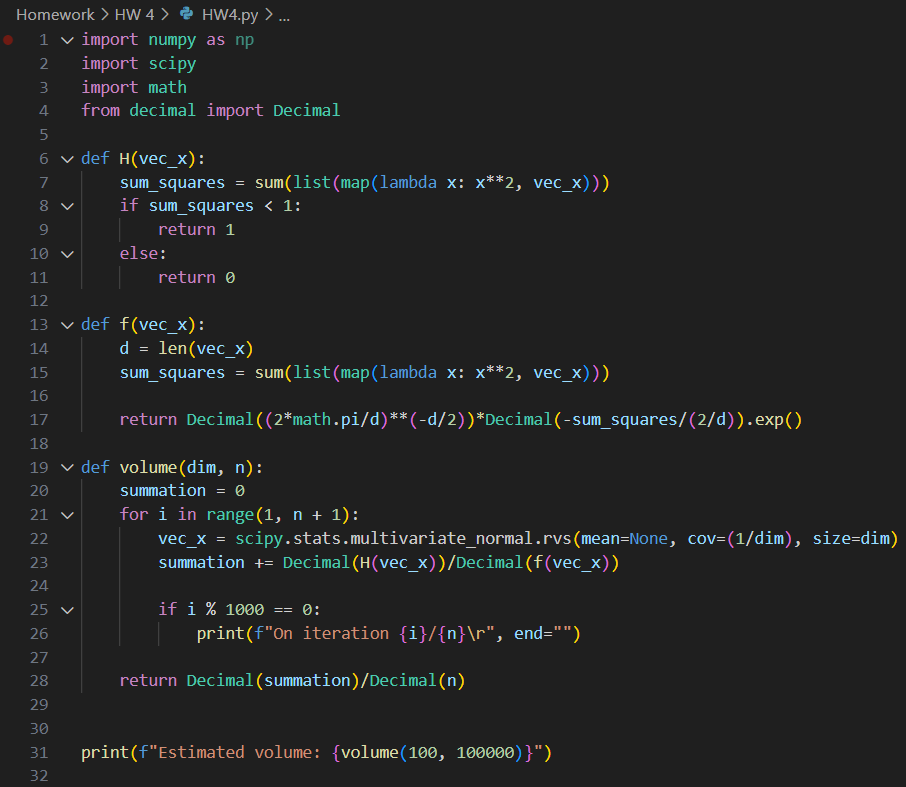
\includegraphics{Images/2B.png}
                    \color{black}
            \end{enumerate}

    \pagebreak
    \item (4 points) Let $\{X_n\}_{n=0}^\infty$ be a homogeneous Markov chain with a discrete state space $\mathcal{X}$. Let $\mu$ denote the PMF of $X_0$, i.e., $\mu(x)=\mathbb{P}(X_0=x)$, for all $x\in\mathcal{X}$; furthermore, $p(x,y)$ denotes the transition probability of the Markov chain, i.e., 
        \begin{align*}
            p(x,y)=\mathbb{P}(X_{n+1}=y\,\vert \, X_n=x)=\mathbb{P}(X_{1}=y\,\vert \, X_0=x),\ \ \mbox{ for all }x,y\in\mathcal{X}.
        \end{align*}
        Prove the following identity
        \begin{align*}
            \mathbb{P}(X_0=x_0, X_1=x_1,\ldots, X_n=x_n)=\mu(x_0)\cdot p(x_0, x_1)\cdot p(x_1, x_2)\ldots p(x_{n-1}, x_n),
        \end{align*}
        for all $n=1,2,\ldots$ and $x_0,x_1,\ldots,x_n\in\mathcal{X}$. (Hint: use the \href{https://en.wikipedia.org/wiki/Law_of_total_probability}{law of total probability}/definition of \href{https://en.wikipedia.org/wiki/Conditional_probability}{conditional probability}, and the Markov property in Eq.~\eqref{eq: Markov property for general MC}.)
    
        \color{blue}           
            By the law of total probability and the Markov property,
            \begin{align*}
                \mathbb{P}(X_0=x_0, \ldots, X_n=x_n) &= \P(X_n = x_n \; | \; X_{n-1} = x_{n-1}, \dots, \; X_0 = x)\cdot \P(X_{n-1} = x_{n-1}, \dots, \; X_0 = x)\\
                &= \P(X_{n} = x_{n} \; | \; X_{n-1} = x_{n-1}) \cdot \P(X_{n-1} = x_{n-1}, \dots, \; X_0 = x)\\
                &= p(x_{n-1}, x_n) \cdot \P(X_{n-1} = x_{n-1}, \dots, \; X_0 = x)\\
                &= p(x_{n-1}, x_n) \cdot p(x_{n-1}, x_{n-2}) \dots \P(X_1 = x_1, X_0 = x_0)\\
                &= p(x_{n-1}, x_n) \cdot p(x_{n-1}, x_{n-2}) \dots \P(X_1 = x_1 \; | \; X_0 = x_0) \cdot \P(X_0 = x_0)\\
                &= p(x_{n-1}, x_n) \cdot p(x_{n-2}, x_{n-1}) \dots p(x_0, x_1) \cdot \mu(x_0)\\
                &= \mu(x_0)\cdot p(x_0, x_1)\cdot p(x_1, x_2)\ldots p(x_{n-1}, x_n) \qed
            \end{align*}
        \color{black}
\end{enumerate}

%\bibliographystyle{plain}
\bibliography{sample}


\end{document}
